\begin{SCfigure} \label{fig:dna_encoding}
  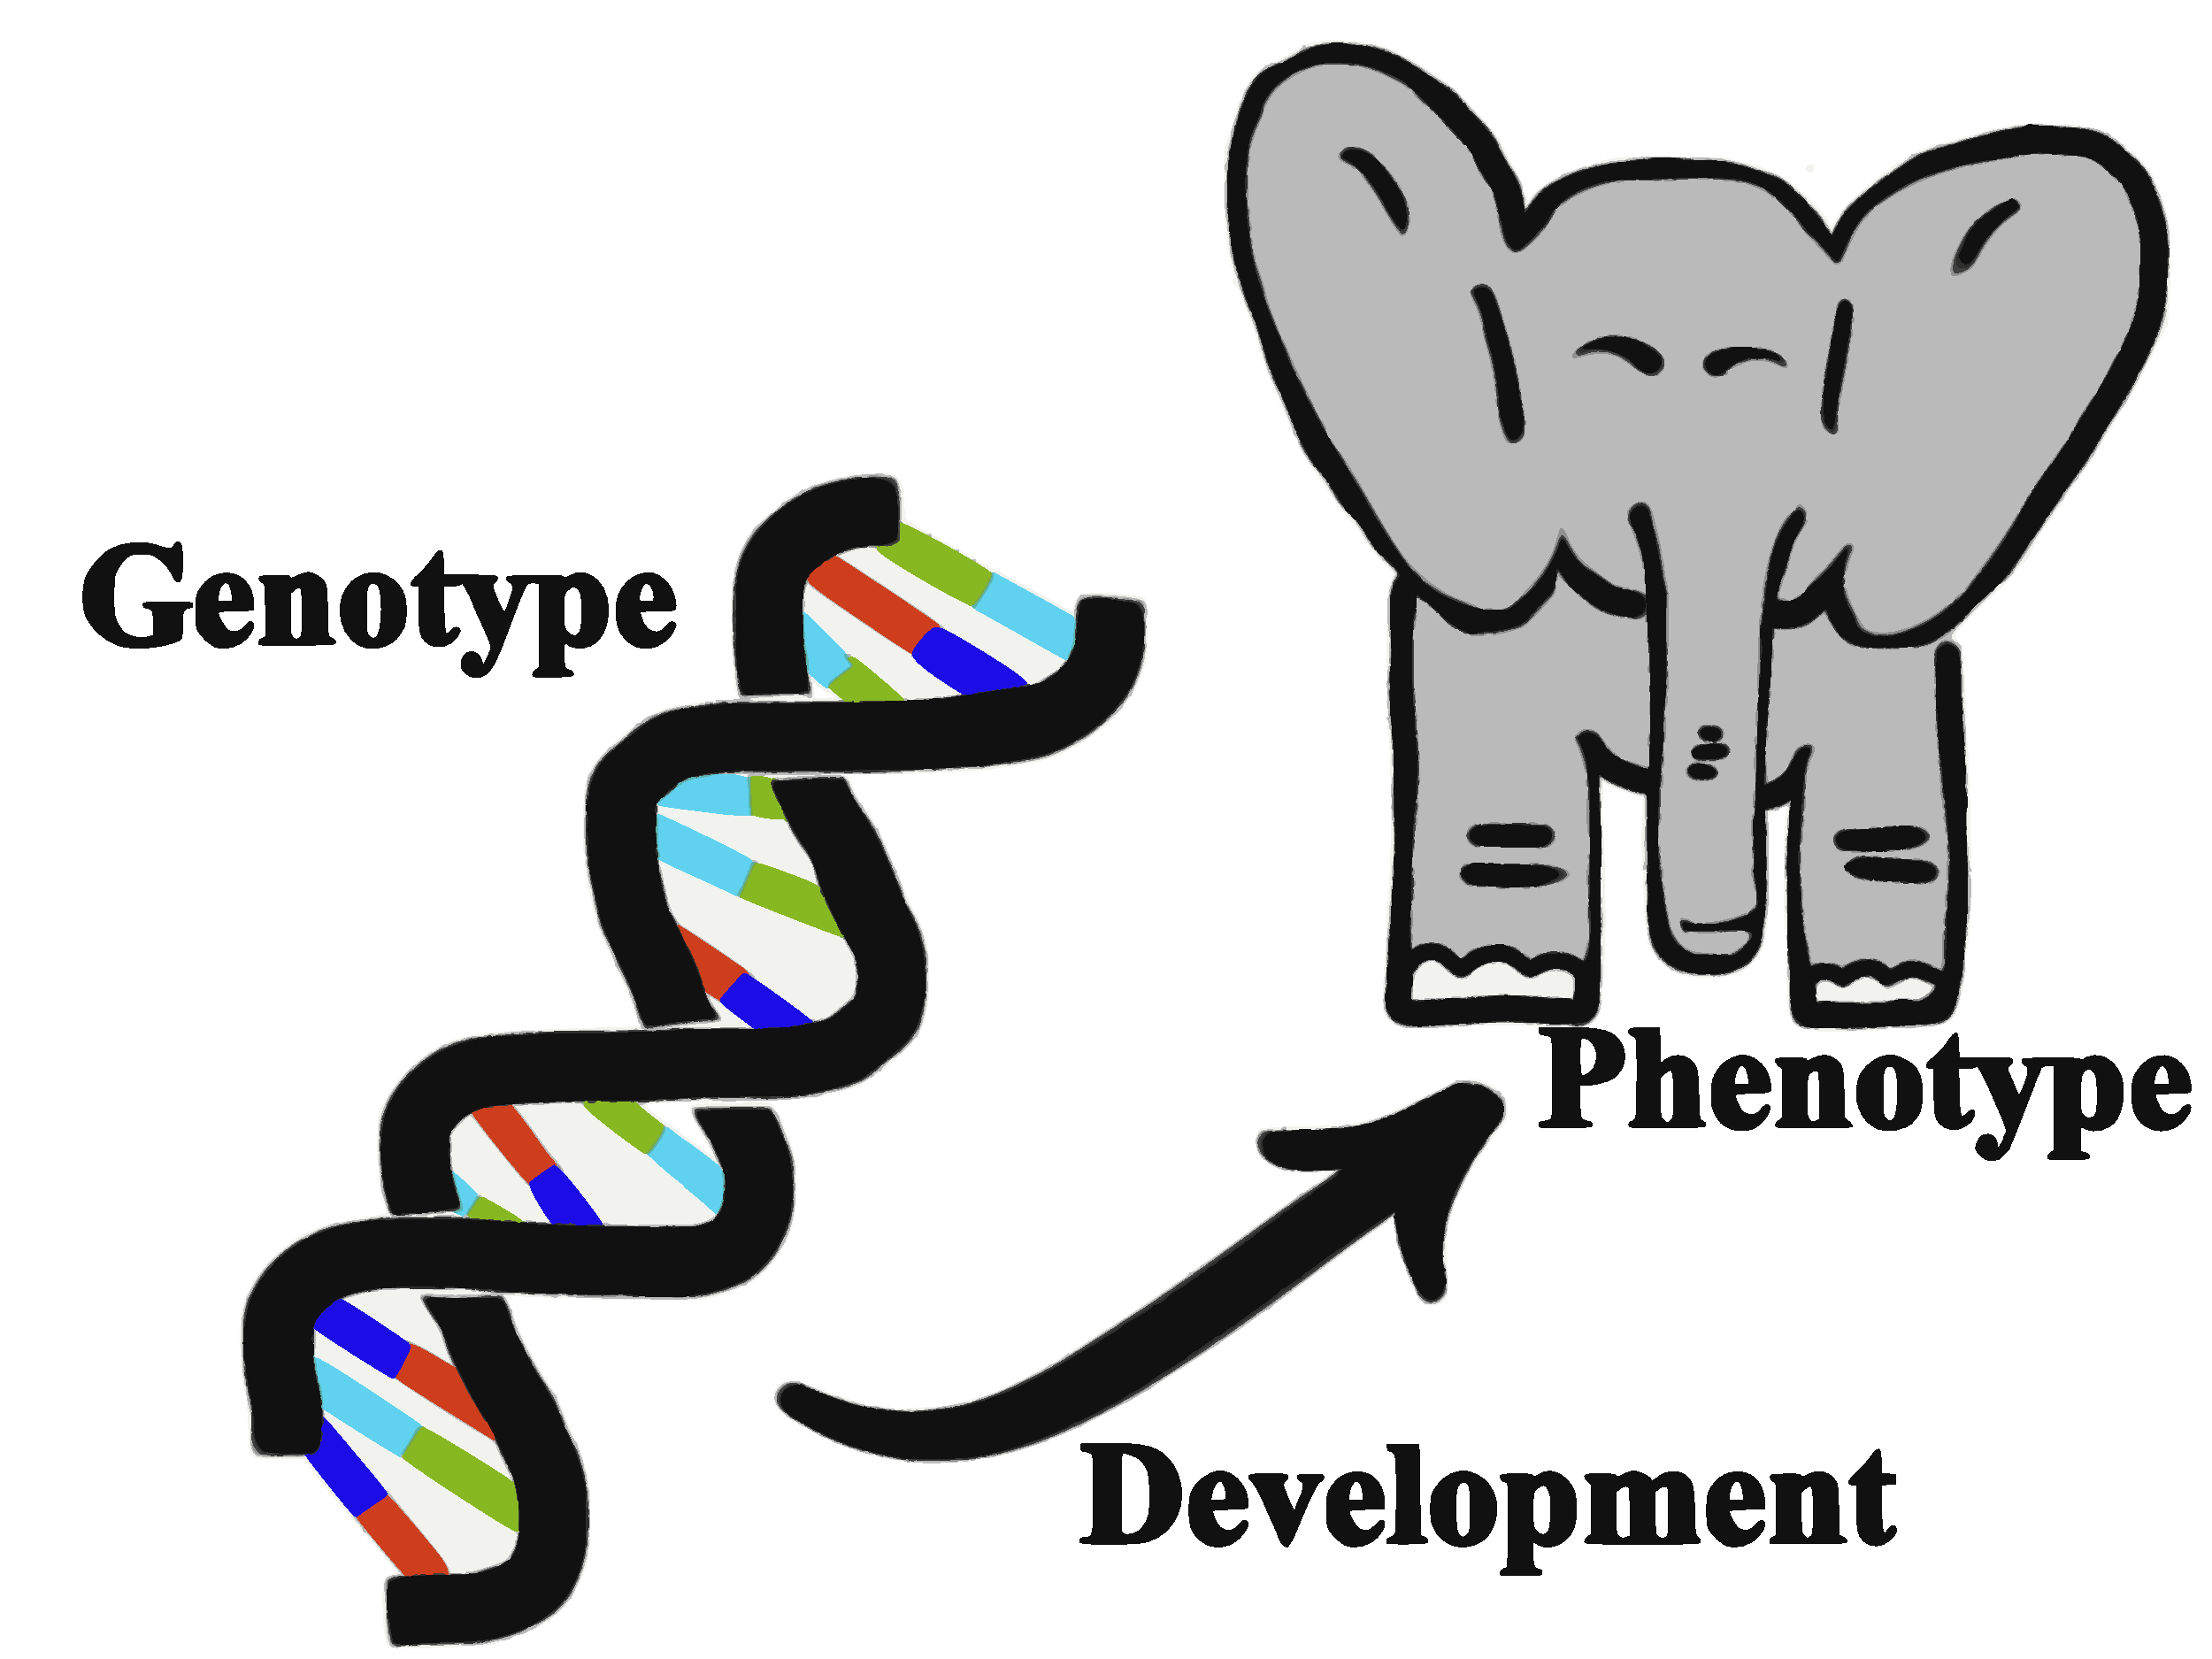
\includegraphics[width=0.7\textwidth]{img/dna_encoding}
  %\captionsetup{singlelinecheck=off,justification=raggedright}

  \caption[Illustration of Indirect Genetic Encoding in an Elephant]{This cartoon illustrates principle of indirect encoding by juxtaposing the genotype and phenotype of the elephant. In the case of an elephant, the genotype is comprised of approximately \num{5e9} base pairs and the phenotype is comprised of approximately \num{1e15} cells. Note how the much more information is required to describe the phenotype than the genotype \cite{Kim2011HowBody,Hofreiter2008MammothGenetics}.}
\end{SCfigure}